\documentclass[UTF8]{article}
\usepackage{ctex}
\usepackage{verbatim}
%\usepackage{amsmath}
\usepackage{graphicx}
\usepackage{palatino}
\usepackage{tikz}
\usetikzlibrary{shapes.geometric, arrows}

\title{\heiti 模电基础}
\author{\heiti 庄梓伸}
\date{\heiti \today}

\begin{document}
\maketitle

\section{PN结}

\section{二极管}

\section{三极管}

\subsection{三极管的结构}

\subsection{三极管的放大作用原理}
三极管有四种工作状态：放大、饱和、截止、倒置。
在工程中，我们最常用的是三极管的放大状态，常通过三极管的放大作用来实现电流的放大，那么三极管是如何将电流放大的呢？

首先我们要知道，无论是PNP三极管，还是NPN三极管，只有在三极管的发射结加上正向偏置电压，在集电结上加反向偏置电压（如图），三极管才能进入放大状态
我们以NPN管为例，将三极管等效成一个三端口网络，我们研究三端电流的产生原因。

\begin{figure}[ht]
    
    \centering
    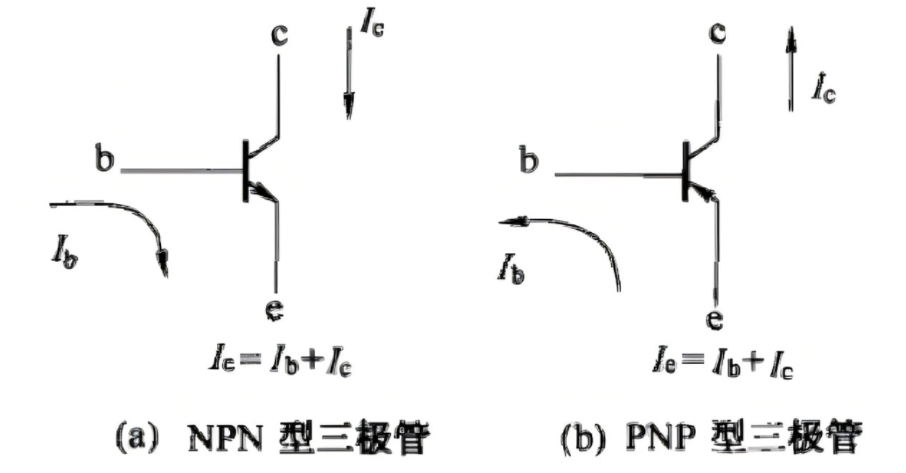
\includegraphics[scale=0.3]{Pic/三极管放大状态电流.png}
    \caption{三极管放大状态电流}
    \label{fig:label}
\end{figure}
\begin{comment}
\thispagestyle{empty}
% 流程图定义基本形状
\tikzstyle{rectangle} = [rectangle, minimum width=3cm, minimum height=1cm, text centered, draw=black]
% 箭头形式
\tikzstyle{arrow} = [->,>=stealth]

%tikz绘图
\begin{tikzpicture}[node distance=0.5cm]
    %定义流程图具体形状
    \node[rectangle](0){be间正向电压};
    \node[rectangle, below of = 0, yshift = -1cm](1){e区电子流向b区产生电子扩散电流$I_{EN}$,b区空穴流向e区产生空穴扩散电流$I_{EP}$};
    \node[rectangle, below of = 1, yshift = -1cm](2){发射极电流$I_{E}=I_{EP}+I_{EN}$};
    \node[rectangle, below of = 2, yshift = -1cm](3){$I_{E}=I_{EP}+I_{EN}$};
    \node[rectangle, below of = 3, yshift = -1cm](4){Process 2};
    \node[rectangle, below of = 4, yshift = -1cm](5){Output};
    \node[rectangle, below of = 5, yshift = -1cm]6){Stop};
    %\coordinate (point1) at (-3cm, -6cm);
    %连接具体形状
    \draw [arrow] (0) -- (1);
    \draw [arrow] (1) -- (2);
    \draw [arrow] (2) -- (3);
    \draw [arrow] (3) -- node [right] {N} (4);
    \draw [arrow] (4) -- (5);
    \draw [arrow] (5) -- (6);
\end{tikzpicture}


\begin{enumerate}
    \item $I_{E}$的产生
    $$be间正向电压 \rightarrow e区电子流向b区产生电子扩散电流I_{EN},b区空穴流向e区产生空穴扩散电流I_{EP} \rightarrow 发射极电流I_{E}=I_{EP}+I_{EN} \overset{11}{\rightarrow} x(-a(t\mp \frac{b}{a}))$$
\end{enumerate}
\end{comment}

\end{document}